\chapter{De la mécanique des particules aux champs classiques}

\section{Qu’est-ce qu’un champ ?}

Le cours précédent a développé la mécanique relativiste des particules à partir d’une action invariante. Nous changeons maintenant d’objet dynamique. Le sujet est la théorie classique des champs, et non la théorie quantique des champs. La mécanique quantique fournira parfois des comparaisons utiles, mais les équations de ce chapitre décrivent des champs classiques ordinaires. L’électromagnétisme constitue le modèle familier en arrière-plan : les ondes électromagnétiques se propagent dans l’espace et interagissent avec les particules chargées. Nous commencerons par un champ encore plus simple.

Un espace-temps peut avoir de nombreuses coordonnées spatiales, mais une seule coordonnée temporelle. Écrivons
\begin{equation}
x^\mu=(t,x^1,\ldots,x^d),
\end{equation}
où l’indice spatial \(i=1,\ldots,d\). Le nombre \(d\) peut être égal à trois, comme dans notre monde, ou à un, deux, neuf, vingt-cinq, ou à toute autre valeur utile à un modèle. À ce stade, l’asymétrie essentielle est qu’il n’existe toujours qu’une seule direction temporelle. Le cours ne cherche pas à expliquer pourquoi les théories comportant plusieurs temps sont si difficiles ; il adopte simplement le cadre à un seul temps dans lequel s’élabore la physique causale ordinaire.

Un champ est une grandeur mesurable dont la valeur peut varier d’un point à l’autre et au cours du temps. La température en est un exemple simple :
\begin{equation}
T=T(\mathbf{x},t).
\end{equation}
Elle associe un nombre à chaque événement ; c’est donc un champ scalaire. La vitesse du vent varie elle aussi dans l’espace et au cours du temps, mais elle a une norme et une direction, et possède donc plusieurs composantes : c’est un champ vectoriel. En physique relativiste, les vecteurs naturels ont quatre composantes plutôt que trois.

Dans la majeure partie de ce cours, le champ a une composante et est désigné par la lettre grecque correspondant à \(f\) :
\begin{equation}
\phi=\phi(\mathbf{x},t).
\label{eq:sr4-field-definition}
\end{equation}
Dire que \(\phi\) est un scalaire signifiera, à terme, davantage que le fait qu’il n’a qu’une seule composante. Cela signifiera que tous les observateurs inertiels attribuent la même valeur à \(\phi\) au même événement physique. Cette loi de transformation n’interviendra qu’une fois la mécanique variationnelle établie.

\section{Le modèle de la particule}

\subsection{Une coordonnée appelée \texorpdfstring{\(\phi\)}{phi}}

Le chemin le plus rapide vers la théorie des champs consiste à revenir à une particule non relativiste ordinaire. Supposons que la particule se déplace sur une ligne, mais appelons sa coordonnée \(\phi\) au lieu de \(x\). Rien en mathématiques n’impose de nommer une coordonnée \(x\) ; ce nom inhabituel est choisi pour rendre visible l’analogie à venir. Traçons le temps horizontalement. L’histoire complète de la particule est alors une courbe \(\phi(t)\), qui peut prendre des valeurs positives comme négatives.

Pour des temps initial et final fixés \(a\) et \(b\), l’action vaut
\begin{align}
A[\phi]
&=\int_a^b dt\,L(\phi,\dot\phi),\\
L(\phi,\dot\phi)
&=\frac{m}{2}\dot\phi^{\,2}-V(\phi).
\label{eq:sr4-particle-lagrangian}
\end{align}
L’équation d’Euler--Lagrange est
\begin{equation}
\frac{d}{dt}\left(\frac{\partial L}{\partial\dot\phi}\right)
-\frac{\partial L}{\partial\phi}=0.
\label{eq:sr4-particle-el}
\end{equation}
Pour le lagrangien de \eqref{eq:sr4-particle-lagrangian},
\begin{equation}
\frac{\partial L}{\partial\dot\phi}=m\dot\phi,
\qquad
\frac{\partial L}{\partial\phi}=-\frac{dV}{d\phi},
\end{equation}
d’où
\begin{equation}
\boxed{m\ddot\phi=-\frac{dV}{d\phi}}.
\label{eq:sr4-newton}
\end{equation}
Il s’agit simplement de l’équation de Newton, écrite avec \(\phi\) comme coordonnée.

\begin{figure}[htbp]
\centering
\includegraphics[width=0.90\textwidth]{lecture_04_figure_01.png}
\caption{L’équation ordinaire d’Euler--Lagrange et son résultat newtonien pour la coordonnée \(\phi(t)\).}
\lectureframe{00:10:18}
\end{figure}

La trajectoire physique rend l’action stationnaire lorsque les extrémités sont maintenues fixes. Le cours dit souvent \emph{minimum}, mais l’énoncé précis est celui de la stationnarité : la trajectoire peut correspondre à un minimum, à un maximum ou à une autre valeur stationnaire. On peut se représenter la situation en divisant l’intervalle de temps en un grand nombre de petits morceaux. L’action devient alors une fonction des nombreuses valeurs échantillonnées de \(\phi\). Faire varier ces valeurs en laissant fixes les extrémités, puis dériver par rapport à chacune d’elles, constitue l’ancêtre en dimension finie de l’équation d’Euler--Lagrange.

\subsection{La mécanique comme théorie en dimensions \texorpdfstring{\(0+1\)}{0+1} }

Imaginons maintenant un monde avec du temps, mais sans dimension spatiale. Son espace se réduit à un point. Un champ dans ce monde ne peut dépendre de la position, puisqu’il n’y a pas de position dont il puisse dépendre ; il ne peut être qu’une fonction \(\phi(t)\). La mécanique ordinaire d’une particule à une coordonnée peut donc se lire comme une théorie des champs en dimensions \(0+1\). Les mathématiques n’ont pas changé. Seule l’interprétation passe de la position d’une particule à la valeur d’un champ dans un monde sans espace.

\begin{figure}[htbp]
\centering
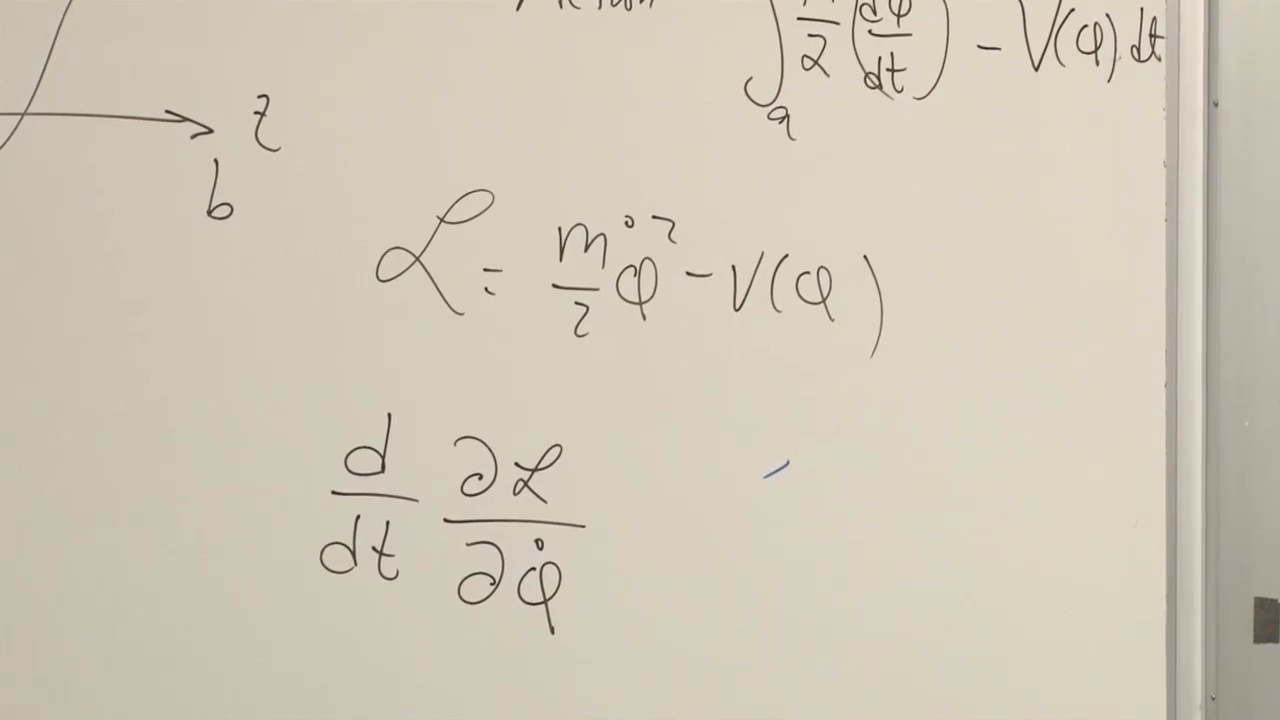
\includegraphics[width=0.90\textwidth]{lecture_04_figure_02.png}
\caption{L’histoire échantillonnée \(\phi(t)\) : une trajectoire de particule et, selon une nouvelle interprétation, l’histoire d’un champ en dimensions \(0+1\).}
\lectureframe{00:14:30}
\end{figure}

\begin{classroomqa}
\audiencequestion{Le potentiel disparaît-il en l’absence de dimensions spatiales ?}
\lecturerresponse{Non. La variation spatiale disparaît, mais le champ conserve une valeur. L’énergie peut dépendre de cette valeur par l’intermédiaire de \(V(\phi)\). Dans l’interprétation en termes de particule, déplacer la courbe vers le haut ou vers le bas modifie l’énergie potentielle ; dans celle en termes de champ, différentes valeurs de \(\phi\) correspondent à différentes énergies potentielles. \lecturetimestamp{00:15:00}}
\end{classroomqa}

\begin{classroomqa}
\audiencequestion{Au lieu d’imaginer un monde entièrement dépourvu d’espace, peut-on imaginer un espace ordinaire dans lequel le champ ne dépend que du temps ?}
\lecturerresponse{Oui. Pour ce propos, les mathématiques locales sont les mêmes : toutes les dérivées spatiales s’annulent et seul \(\phi(t)\) subsiste. Parler d’une théorie en dimensions \(0+1\) permet d’isoler cette structure réduite, mais un champ spatialement homogène dans un monde de dimension supérieure donne la même intuition. \lecturetimestamp{00:16:25}}
\end{classroomqa}

Le détour prend maintenant tout son sens. Nous connaissons le principe de l’action pour un champ qui dépend d’une seule coordonnée, le temps. Nous pouvons nous appuyer sur ce schéma pour deviner le principe de l’action d’un champ qui dépend de toutes les coordonnées de l’espace-temps.

\section{L’histoire d’un champ dans l’espace-temps}

\subsection{D’une courbe à une surface}

En dimensions \(1+1\), l’espace-temps est lui-même un plan de coordonnées \(t\) et \(x\). La valeur \(\phi(x,t)\) fournit une troisième direction. L’histoire du champ est donc une surface au-dessus du plan de l’espace-temps, et non une courbe. Cette surface peut s’élever au-dessus de zéro ou passer en dessous, car un champ scalaire n’est pas nécessairement positif.

\begin{figure}[htbp]
\centering
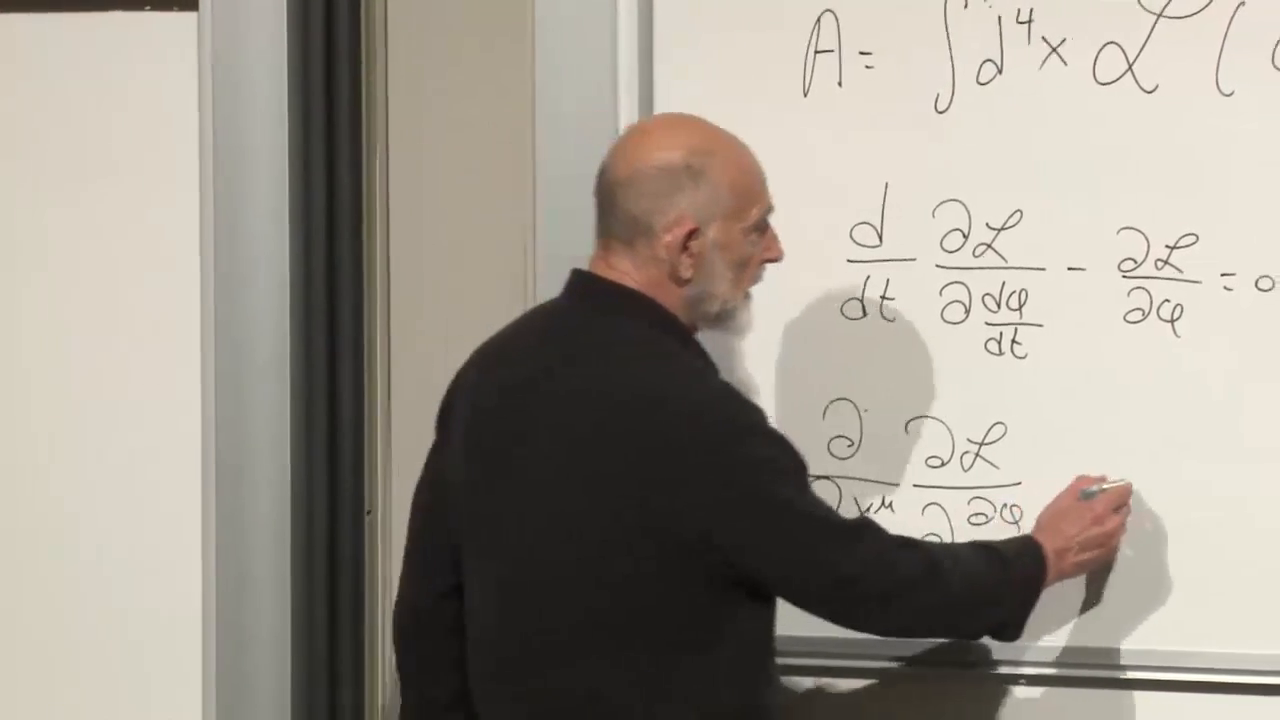
\includegraphics[width=0.90\textwidth]{lecture_04_figure_03.png}
\caption{L’histoire d’un champ scalaire représentée par une surface au-dessus d’un plan d’espace-temps en dimensions \(1+1\).}
\lectureframe{00:20:46}
\end{figure}

Notre espace-temps physique est dit de dimension \(3+1\) : trois dimensions d’espace et une de temps. Un modèle de table est en dimensions \(2+1\), et des perles contraintes à se déplacer le long d’un fil évoquent un monde en dimensions \(1+1\). L’axe supplémentaire nécessaire pour représenter \(\phi\) rend même le cas \(3+1\) impossible à dessiner fidèlement. La définition, elle, ne laisse aucune ambiguïté : une histoire complète associe une valeur de \(\phi\) à chaque événement de l’espace-temps.

\subsection{Des extrémités fixes aux données fixées sur la frontière}

Le problème variationnel d’une particule consiste à fixer deux extrémités et à faire varier la courbe entre elles. Son analogue en théorie des champs consiste à choisir une région de l’espace-temps, à fixer \(\phi\) sur sa frontière et à faire varier \(\phi\) à l’intérieur. La région peut être un rectangle sur un dessin en dimensions \(1+1\), ou toute région appropriée dans un espace-temps de dimension supérieure.

\begin{figure}[htbp]
\centering
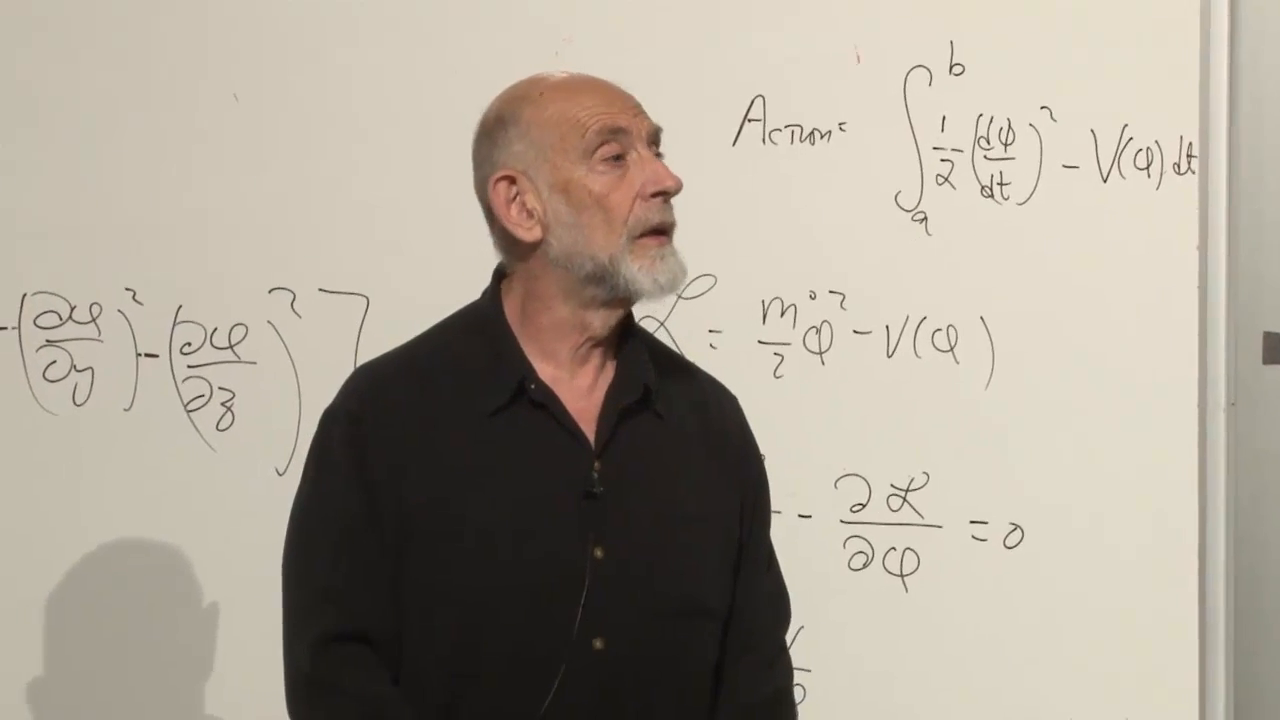
\includegraphics[width=0.90\textwidth]{lecture_04_figure_04.png}
\caption{Une région de l’espace-temps dont toute la frontière est maintenue fixe tandis que le champ varie à l’intérieur.}
\lectureframe{00:24:52}
\end{figure}

\begin{classroomqa}
\audiencequestion{La formulation lagrangienne reste-t-elle valable lorsqu’un potentiel dépend explicitement du temps ?}
\lecturerresponse{Oui. Les formulations d’Euler--Lagrange et hamiltonienne restent valables. En général, c’est la conservation de l’énergie qui disparaît : une dépendance explicite au temps brise la symétrie par translation temporelle. En théorie des champs, l’énoncé correspondant est qu’une dépendance explicite à l’espace-temps est permise, même si elle influe sur les lois de conservation associées. \lecturetimestamp{00:23:49}}
\end{classroomqa}

\begin{classroomqa}
\audiencequestion{Dans la région rectangulaire du champ, fixe-t-on seulement le haut et le bas, ou bien toute la frontière ?}
\lecturerresponse{Pour cette construction variationnelle, c’est toute la frontière qui est fixe : les quatre côtés du rectangle en dimensions \(1+1\). Le champ ne peut varier qu’à l’intérieur. C’est l’analogue direct du maintien des deux extrémités fixes en mécanique des particules. \lecturetimestamp{00:24:24}}
\end{classroomqa}

Fixer toute la frontière est une condition portant sur la variation utilisée pour déduire les équations. Lorsqu’on traite ensuite l’équation hyperbolique du champ comme un problème d’évolution physique, on spécifie plus couramment des données initiales appropriées et on laisse l’équation les faire évoluer dans le temps.

\section{L’action et l’équation d’Euler--Lagrange du champ}

\subsection{La densité lagrangienne}

Divisons la région de l’espace-temps en petites cellules. On suppose que l’action est une somme de contributions locales, une par cellule. Dans la limite continue, cette somme devient une intégrale sur l’espace-temps :
\begin{equation}
A[\phi]
=
\int_{\Omega} d^4x\,
\mathcal{L}\!\left(
\phi,\partial_\mu\phi;x^\mu
\right),
\qquad
d^4x=dt\,dx\,dy\,dz.
\label{eq:sr4-field-action}
\end{equation}
La quantité \(\mathcal{L}\) est la densité lagrangienne. Le point-virgule dans \(\mathcal{L}(\phi,\partial_\mu\phi;x^\mu)\) sépare les arguments dynamiques d’une éventuelle dépendance explicite aux coordonnées. Dans un système fermé homogène, cette dernière dépendance est normalement absente, mais le formalisme variationnel ne l’interdit pas.

La notation compacte
\begin{equation}
\partial_\mu\phi
\equiv
\frac{\partial\phi}{\partial x^\mu}
\end{equation}
rassemble les dérivées temporelle et spatiales. Dans la notation en composantes utilisée dans le cours, on peut aussi écrire
\begin{equation}
\begin{aligned}
\phi_t&=\frac{\partial\phi}{\partial t},\\
\phi_x&=\frac{\partial\phi}{\partial x},\\
\phi_y&=\frac{\partial\phi}{\partial y},\\
\phi_z&=\frac{\partial\phi}{\partial z}.
\end{aligned}
\label{eq:sr4-component-derivatives}
\end{equation}
Il peut y avoir plusieurs champs, tout comme une particule peut avoir plusieurs coordonnées. Pour l’instant, il n’y a qu’un seul champ \(\phi\).

Le symbole \(d^4x\) n’est qu’une abréviation pour la mesure sur les quatre coordonnées. Dans un espace-temps de dimension différente, on le remplacerait par \(d^Dx\). Dans le modèle en dimensions \(0+1\), \(D=1\) et \(d^1x\) est simplement égal à \(dt\).

\begin{figure}[htbp]
\centering
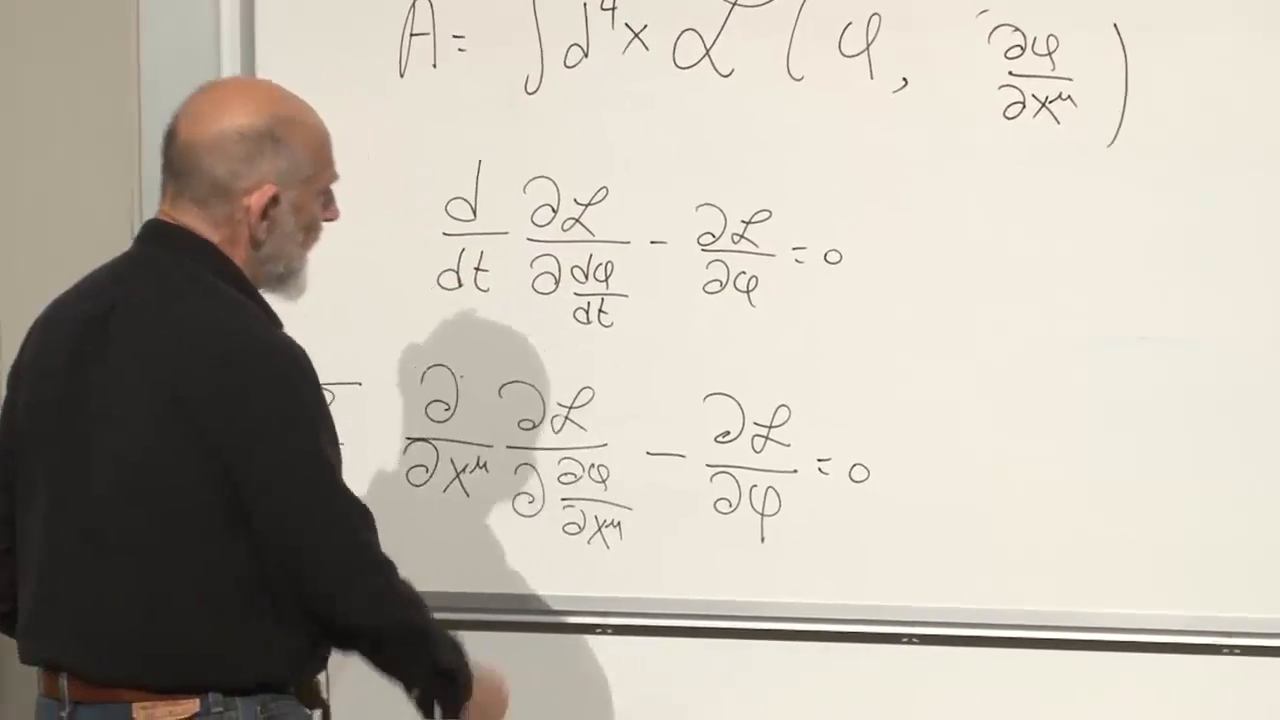
\includegraphics[width=0.90\textwidth]{lecture_04_figure_05.png}
\caption{La densité d’action écrite comme une fonction locale de \(\phi\) et de ses dérivées dans l’espace-temps.}
\lectureframe{00:32:51}
\end{figure}

\begin{classroomqa}
\audiencequestion{La densité lagrangienne peut-elle aussi dépendre de \(x,y,z\) elles-mêmes ?}
\lecturerresponse{Oui, tout comme le lagrangien d’une particule peut dépendre explicitement de \(t\). En général, ce n’est pas le cas dans un système fermé invariant par translation, mais une dépendance explicite aux coordonnées n’invalide pas le formalisme. \lecturetimestamp{00:30:29}}
\end{classroomqa}

\begin{classroomqa}
\audiencequestion{La construction présentée jusqu’ici concerne-t-elle spécifiquement un champ scalaire, ou est-elle générale ?}
\lecturerresponse{Jusqu’ici, le schéma variationnel est général. Le fait de n’écrire qu’une seule composante suggère un champ scalaire. Un champ vectoriel ou un ensemble de champs comporterait des indices de composante supplémentaires, et il faudrait faire varier chaque composante. \lecturetimestamp{00:31:00}}
\end{classroomqa}

\subsection{Le modèle du réseau}

Sur un réseau fin dans l’espace-temps, les dérivées deviennent des différences finies entre les valeurs du champ en des points voisins. L’action est alors une fonction ordinaire de nombreuses variables. Une grille de dix points dans une direction et de huit dans l’autre comporte déjà quatre-vingts variables de champ. Le raffinement de la grille augmente leur nombre, mais la règle de minimisation reste élémentaire : dériver l’action par rapport à la valeur du champ en chaque point intérieur et égaler le résultat à zéro.

\begin{figure}[htbp]
\centering
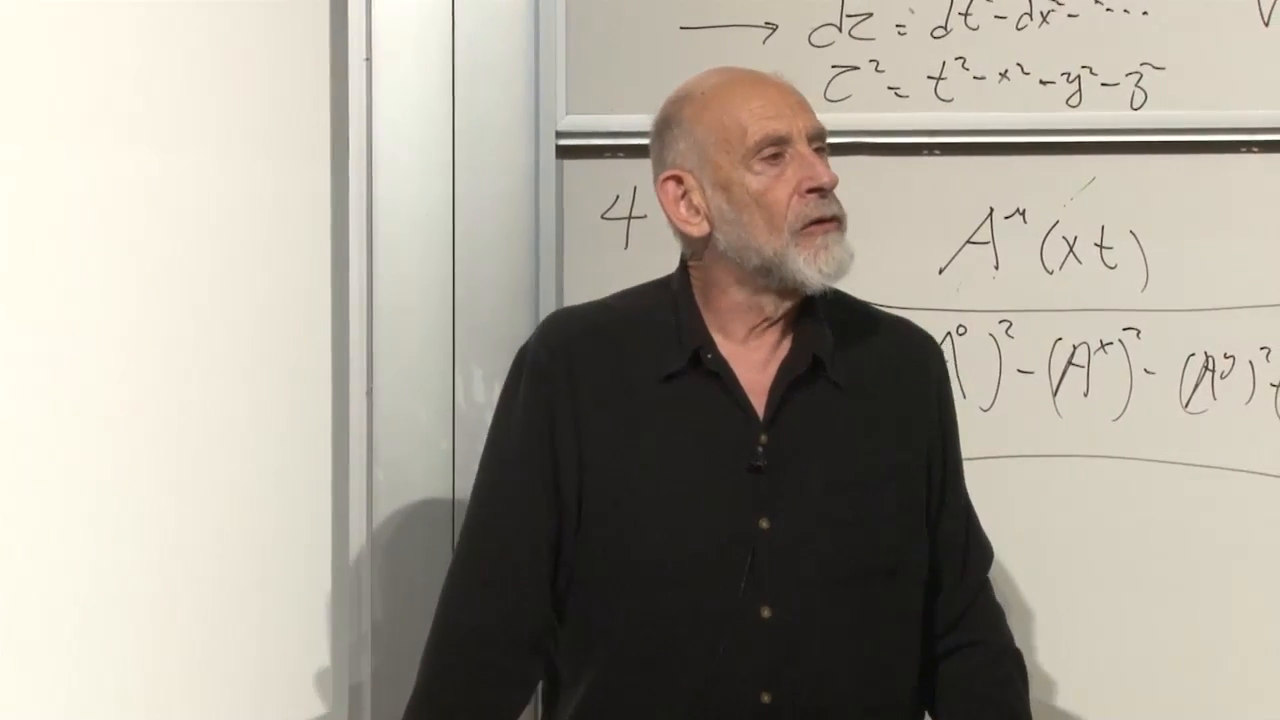
\includegraphics[width=0.90\textwidth]{lecture_04_figure_06.png}
\caption{La région de l’espace-temps divisée en cellules ; avant de passer à la limite continue, l’action est une fonction ordinaire de nombreuses variables.}
\lectureframe{00:34:05}
\end{figure}

Le passage à la limite continue donne l’équation d’Euler--Lagrange du champ,
\begin{equation}
\boxed{
\partial_\mu
\left[
\frac{\partial\mathcal{L}}
{\partial(\partial_\mu\phi)}
\right]
-
\frac{\partial\mathcal{L}}{\partial\phi}
=0
}.
\label{eq:sr4-field-el}
\end{equation}
L’indice \(\mu\) est répété et implique une somme sur toutes les directions de l’espace-temps. Sans cette convention de sommation, la même équation s’écrit
\begin{align}
&
\frac{\partial}{\partial t}
\left(\frac{\partial\mathcal{L}}{\partial\phi_t}\right)
+
\frac{\partial}{\partial x}
\left(\frac{\partial\mathcal{L}}{\partial\phi_x}\right)
+
\frac{\partial}{\partial y}
\left(\frac{\partial\mathcal{L}}{\partial\phi_y}\right)
\nonumber\\
&\hspace{3em}
+
\frac{\partial}{\partial z}
\left(\frac{\partial\mathcal{L}}{\partial\phi_z}\right)
-
\frac{\partial\mathcal{L}}{\partial\phi}
=0.
\label{eq:sr4-field-el-expanded}
\end{align}
Le premier terme est celui que l’on connaît pour une particule. La théorie des champs ajoute un terme analogue pour chaque direction spatiale. Le dernier terme,
\(-\partial\mathcal{L}/\partial\phi\), reste inchangé.

\begin{figure}[htbp]
\centering
\includegraphics[width=0.90\textwidth]{lecture_04_figure_07.png}
\caption{L’équation d’Euler--Lagrange en une dimension et sa généralisation à l’espace-temps, présentées l’une sous l’autre.}
\lectureframe{00:38:44}
\end{figure}

On appelle aussi ce domaine la mécanique des milieux continus. Selon les degrés de liberté, les mêmes mathématiques peuvent décrire l’écoulement d’un fluide, la déformation élastique ou un autre milieu continu.

\begin{classroomqa}
\audiencequestion{Les mêmes équations fonctionneraient-elles dans un monde avec de l’espace, mais sans temps ?}
\lecturerresponse{Oui, comme problème variationnel purement spatial. Physiquement, c’est ainsi que l’on cherche une solution statique : on suppose que le champ ne dépend pas du temps, on élimine toutes les dérivées temporelles et on résout les équations spatiales restantes. Une configuration électrique ou magnétique indépendante du temps en est un exemple. \lecturetimestamp{00:40:05}}
\end{classroomqa}

\section{Deviner la dynamique scalaire la plus simple}

\subsection{Pourquoi les signes ne peuvent pas tous être identiques}

Reprenons le terme cinétique de la particule \(\tfrac12\dot\phi^2\), posons son coefficient global non pertinent égal à un et essayons de le généraliser. Une première conjecture pourrait être
\begin{equation}
\mathcal{L}_{+}
=
\frac12
\left[
\phi_t^2+\phi_x^2+\phi_y^2+\phi_z^2
\right].
\label{eq:sr4-all-plus}
\end{equation}
Ce détour est utile, même s’il mène à une erreur. Cette expression traite le temps et l’espace avec des signes identiques. L’équation qui en résulterait n’aurait pas la structure hyperbolique de la propagation des ondes. La combinaison relativiste correcte attribue un signe au temps et le signe opposé à l’espace.

\begin{classroomqa}
\audiencequestion{L’expression où tous les signes sont positifs est-elle erronée parce que le lagrangien doit être invariant relativiste ?}
\lecturerresponse{C’est la réponse la plus profonde, et elle est juste. Le cours parvient d’abord au choix du signe de façon plus élémentaire : les ondes distinguent l’évolution dans le temps de la variation dans l’espace, de sorte que le temps ne peut pas intervenir exactement comme une coordonnée spatiale supplémentaire. L’invariance de Lorentz donnera bientôt à cette intuition une formulation précise. \lecturetimestamp{00:43:19}}
\end{classroomqa}

En rétablissant une vitesse caractéristique \(c\), la densité lagrangienne scalaire la plus simple est
\begin{equation}
\boxed{
\mathcal{L}
=
\frac12
\left[
\frac{1}{c^2}\phi_t^2
-\phi_x^2-\phi_y^2-\phi_z^2
\right]
-V(\phi)
}.
\label{eq:sr4-scalar-lagrangian}
\end{equation}
Pour un champ relativiste, \(c\) est la vitesse de la lumière. Dans un modèle de milieu continu, elle pourrait plutôt être la vitesse du son, celle d’une onde élastique ou une autre vitesse caractéristique de propagation.

Le facteur global \(1/2\) est une convention, comme dans \(\tfrac12m\dot\phi^2\). Multiplier toute une action par une constante non nulle ne modifie pas ses trajectoires stationnaires ; cette convention fixe la manière de nommer et de normaliser les paramètres des équations. Une fois cette normalisation choisie, il faut l’appliquer de manière cohérente.

\begin{classroomqa}
\audiencequestion{Peut-on considérer les termes de gradient spatial comme faisant partie de l’énergie potentielle ?}
\lecturerresponse{Oui. Dans la décomposition en énergie cinétique moins énergie potentielle, la partie cinétique contient les dérivées temporelles. Les termes sans dérivées temporelles, y compris les gradients spatiaux et \(V(\phi)\), relèvent de l’énergie potentielle. Dans une théorie relativiste, la raison fondamentale de leur signe relatif est la métrique lorentzienne. \lecturetimestamp{00:45:37}}
\end{classroomqa}

\subsection{L’équation d’onde}

Appliquons \eqref{eq:sr4-field-el}. Les termes dérivés valent
\begin{equation}
\frac{\partial\mathcal{L}}{\partial\phi_t}
=\frac{1}{c^2}\phi_t,
\qquad
\frac{\partial\mathcal{L}}{\partial\phi_i}
=-\phi_i,
\end{equation}
tandis que
\begin{equation}
\frac{\partial\mathcal{L}}{\partial\phi}
=-\frac{dV}{d\phi}.
\end{equation}
Par conséquent,
\begin{equation}
\begin{aligned}
&\boxed{
\frac{1}{c^2}\frac{\partial^2\phi}{\partial t^2}
-\nabla^2\phi
+\frac{dV}{d\phi}
=0
},\\[0.5em]
\nabla^2
&=
\frac{\partial^2}{\partial x^2}
+\frac{\partial^2}{\partial y^2}\\
&\quad
+\frac{\partial^2}{\partial z^2}.
\end{aligned}
\label{eq:sr4-general-scalar-eom}
\end{equation}

Si \(V=0\), cette équation se réduit à
\begin{equation}
\boxed{
\frac{1}{c^2}\phi_{tt}-\nabla^2\phi=0
},
\label{eq:sr4-wave-equation}
\end{equation}
l’équation d’onde. Le cours reconnaît l’équation, mais en remet la résolution à plus tard. Ses solutions propagent les perturbations à la vitesse \(c\).

\begin{figure}[htbp]
\centering
\includegraphics[width=0.90\textwidth]{lecture_04_figure_08.png}
\caption{La forme en une dimension \(c^{-2}\phi_{tt}-\phi_{xx}=0\), reconnue comme l’équation d’onde.}
\lectureframe{00:50:30}
\end{figure}

\subsection{Un champ d’oscillateurs harmoniques couplés}

Choisissons maintenant un potentiel quadratique,
\begin{equation}
V(\phi)=\frac12\mu^2\phi^2,
\qquad
\frac{dV}{d\phi}=\mu^2\phi.
\label{eq:sr4-quadratic-potential}
\end{equation}
Si \(\phi\) désignait la position d’une particule, ce serait le potentiel d’un oscillateur harmonique de constante de raideur \(\mu^2\). Pour le champ,
\begin{equation}
\boxed{
\frac{1}{c^2}\phi_{tt}-\nabla^2\phi+\mu^2\phi=0
}.
\label{eq:sr4-klein-gordon}
\end{equation}
Sans la dérivée spatiale, il s’agit simplement de l’accélération plus une constante multipliée par le déplacement, le tout égal à zéro. Le gradient couple les points voisins et transforme l’oscillateur en un milieu continu où des ondes peuvent se propager. En théorie relativiste des champs, \eqref{eq:sr4-klein-gordon} est appelée équation de Klein--Gordon massive ; au niveau classique, \(\mu\) est l’échelle de longueur inverse qui modifie la propagation des ondes.

\begin{figure}[htbp]
\centering
\includegraphics[width=0.90\textwidth]{lecture_04_figure_09.png}
\caption{Le potentiel quadratique et l’équation d’onde qui en résulte, avec le terme de rappel \(\mu^2\phi\).}
\lectureframe{00:52:38}
\end{figure}

\begin{classroomqa}
\audiencequestion{Pourquoi le facteur \(1/2\) dans \(V=\tfrac12\mu^2\phi^2\) disparaît-il de l’équation du mouvement ?}
\lecturerresponse{La dérivation de \(\phi^2\) fournit un facteur deux. Le facteur conventionnel \(1/2\) est précisément introduit pour que \(dV/d\phi=\mu^2\phi\), tout comme \(V(x)=\tfrac12kx^2\) donne la force de rappel \(-kx\). \lecturetimestamp{00:53:17}}
\end{classroomqa}

L’équation est linéaire : \(\phi\) et chacune de ses dérivées n’interviennent qu’à la puissance un. Des termes tels que \(\phi^2\) ou \(\phi\,\partial_\mu\phi\) dans l’équation du mouvement rendraient la dynamique non linéaire.

\section{Scalaires de Lorentz et quadrivecteurs}

\subsection{L’action doit être indépendante du référentiel}

Le formalisme variationnel à lui seul définit de nombreuses théories des champs possibles. La relativité impose en plus que l’action ait la même valeur et la même forme dans tous les référentiels inertiels. Pour la particule libre, cette condition était satisfaite en intégrant le temps propre invariant \(d\tau\) le long de la ligne d’univers. Pour un champ, on intègre l’action sur l’espace-temps ; ses éléments constitutifs locaux doivent donc se transformer de façon appropriée.

Sous une transformation de Lorentz propre, la mesure de l’espace-temps est invariante : \(d^4x'=d^4x\). Il suffit donc d’exiger que la densité lagrangienne soit un scalaire de Lorentz :
\begin{equation}
\mathcal{L}'(x')=\mathcal{L}(x).
\label{eq:sr4-lagrangian-scalar}
\end{equation}

\subsection{Champs scalaires}

Un champ scalaire obéit à
\begin{equation}
\boxed{\phi'(x')=\phi(x)}.
\label{eq:sr4-scalar-transform}
\end{equation}
Les coordonnées \(x\) et \(x'\) désignent le même événement dans deux référentiels. Les expressions fonctionnelles utilisées par les observateurs peuvent sembler différentes, mais le nombre associé à cet événement physique est le même.

\begin{figure}[htbp]
\centering
\includegraphics[width=0.90\textwidth]{lecture_04_figure_10.png}
\caption{Loi de transformation qui définit un champ scalaire : \(\phi(x)=\phi'(x')\).}
\lectureframe{00:59:33}
\end{figure}

La température a fourni l’intuition initiale, même si un thermomètre en mouvement dans un milieu matériel n’est pas un exemple relativiste parfait. C’est la définition \eqref{eq:sr4-scalar-transform}, et non l’analogie avec le thermomètre, qui importe.

\subsection{Quadrivecteurs}

Dans les unités \(c=1\), un boost de vitesse \(v\) selon l’axe \(x\) agit comme suit :
\begin{equation}
\begin{aligned}
t'&=\gamma(t-vx),\\
x'&=\gamma(x-vt),\\
y'&=y,\\
z'&=z,\\
\gamma&=\frac{1}{\sqrt{1-v^2}}.
\end{aligned}
\label{eq:sr4-x-boost}
\end{equation}

\begin{figure}[htbp]
\centering
\includegraphics[width=0.90\textwidth]{lecture_04_figure_11.png}
\caption{Transformation de Lorentz correspondant à un boost selon l’axe \(x\), dans les unités \(c=1\).}
\lectureframe{01:02:26}
\end{figure}

Toute famille de quatre grandeurs qui se mélangent de la même manière sous les boosts forme un quadrivecteur. Parmi les exemples déjà rencontrés figurent \(x^\mu\), \(dx^\mu\) et la quadri-vitesse \(u^\mu=dx^\mu/d\tau\). La multiplication d’un quadrivecteur par un scalaire donne un autre quadrivecteur. Un fluide relativiste en écoulement en fournit un exemple de champ : sa quadri-vitesse \(u^\mu(x)\) peut varier d’un événement à l’autre.

Pour le même boost que dans \eqref{eq:sr4-x-boost}, un quadrivecteur générique obéit à
\begin{equation}
\begin{aligned}
A'^0&=\gamma(A^0-vA^x),\\
A'^x&=\gamma(A^x-vA^0),\\
A'^y&=A^y,\\
A'^z&=A^z.
\end{aligned}
\label{eq:sr4-vector-boost}
\end{equation}

Pour un quadrivecteur générique \(A^\mu=(A^0,A^x,A^y,A^z)\), la norme lorentzienne
\begin{equation}
\boxed{
A_\mu A^\mu
=(A^0)^2-(A^x)^2-(A^y)^2-(A^z)^2
}
\label{eq:sr4-vector-norm}
\end{equation}
est un scalaire. Elle est invariante pour la même raison algébrique que
\begin{equation}
d\tau^2=dt^2-dx^2-dy^2-dz^2
\end{equation}
est invariante. Le cours vient brièvement à manquer de lettres disponibles pour désigner un vecteur générique, puis adopte \(A\), sur la suggestion d’utiliser une flèche \(A\).

\begin{figure}[htbp]
\centering
\includegraphics[width=0.90\textwidth]{lecture_04_figure_12.png}
\caption{Un champ quadrivectoriel générique et la différence lorentzienne de carrés qui définit sa norme invariante.}
\lectureframe{01:09:06}
\end{figure}

\subsection{La dérivée d’un scalaire}

La dérivation d’un scalaire par rapport aux quatre coordonnées de l’espace-temps donne les quatre composantes
\begin{equation}
\partial_\mu\phi
=
\left(
\frac{\partial\phi}{\partial t},
\frac{\partial\phi}{\partial x},
\frac{\partial\phi}{\partial y},
\frac{\partial\phi}{\partial z}
\right)
\qquad(c=1).
\end{equation}
À strictement parler, \(\partial_\mu\phi\) est un covecteur ; la métrique de Minkowski relève son indice pour former \(\partial^\mu\phi\). Cette distinction ne change rien à l’argument en composantes présenté ici, mais elle définit sans ambiguïté la contraction :
\begin{equation}
\boxed{
\partial_\mu\phi\,\partial^\mu\phi
=
\frac{1}{c^2}\phi_t^2
-\phi_x^2-\phi_y^2-\phi_z^2
}.
\label{eq:sr4-derivative-scalar}
\end{equation}

\begin{figure}[htbp]
\centering
\includegraphics[width=0.90\textwidth]{lecture_04_figure_13.png}
\caption{Différence invariante de carrés construite à partir des premières dérivées d’un champ scalaire.}
\lectureframe{01:13:55}
\end{figure}

\begin{classroomqa}
\audiencequestion{Cette combinaison de dérivées est-elle le laplacien ?}
\lecturerresponse{Non. L’invariant présenté est quadratique en les premières dérivées. Le laplacien contient des dérivées spatiales secondes. Les dérivées secondes n’apparaissent qu’après variation de l’action, dans l’équation d’onde. \lecturetimestamp{01:13:22}}
\end{classroomqa}

Le motif de signes dans \eqref{eq:sr4-scalar-lagrangian} s’explique maintenant au lieu d’être deviné. La combinaison cinétique et gradient est le scalaire de Lorentz \(\partial_\mu\phi\,\partial^\mu\phi\). La théorie quadratique la plus simple est donc
\begin{equation}
\mathcal{L}
=
\frac12\partial_\mu\phi\,\partial^\mu\phi
-\frac12\mu^2\phi^2.
\label{eq:sr4-covariant-lagrangian}
\end{equation}

\begin{figure}[htbp]
\centering
\includegraphics[width=0.90\textwidth]{lecture_04_figure_14.png}
\caption{Le lagrangien quadratique complet d’un champ scalaire et son équation linéaire sur le tableau.}
\lectureframe{01:19:12}
\end{figure}

\section{Quelle est l’étendue de cette liberté ?}

Une fois connue la règle de construction des scalaires, de nombreux lagrangiens deviennent possibles. Le champ \(\phi\) est un scalaire ; toute fonction ordinaire \(F(\phi)\) est donc elle aussi un scalaire : \(\phi^2\), \(\phi^3\), \(\cosh\phi\), et ainsi de suite. On peut également introduire des paramètres numériques. Un symbole tel que \(\mu\) peut être ajouté comme coefficient constant ; les seules questions qui restent concernent ses dimensions et son interprétation physique.

\begin{classroomqa}
\audiencequestion{Peut-on introduire une masse dans le lagrangien ?}
\lecturerresponse{Un paramètre constant peut tout à fait y figurer. À ce stade, il faut se demander de quel objet c’est la masse, car \(\mu\) n’est qu’un nombre dans la théorie classique des champs tant que sa signification physique n’a pas été précisée. Dans la théorie relativiste quadratique d’un champ scalaire, il fixe l’échelle de masse ou de longueur inverse. \lecturetimestamp{01:14:16}}
\end{classroomqa}

On peut multiplier des scalaires :
\begin{equation}
F(\phi)\,\partial_\mu\phi\,\partial^\mu\phi
\end{equation}
est invariant de Lorentz. On peut aussi élever au carré le scalaire formé par les dérivées, ce qui produit des puissances supérieures des premières dérivées. On peut également envisager des dérivées d’ordre supérieur, bien que le cours se limite aux champs et à leurs premières dérivées, cadre standard qui donne des équations du mouvement du second ordre. Les théories à dérivées d’ordre supérieur demandent davantage de précautions, car elles introduisent généralement des données dynamiques supplémentaires et des instabilités possibles.

\begin{classroomqa}
\audiencequestion{La construction par différence de carrés est-elle vraiment la métrique de l’espace-temps ?}
\lecturerresponse{Oui. Dans la convention de signature choisie, la métrique est \(dt^2-dx^2-dy^2-dz^2\). Le cours n’a pas encore insisté sur le terme « métrique », mais il s’agit bien de la géométrie de l’espace-temps qui deviendra centrale en relativité générale. \lecturetimestamp{01:19:39}}
\end{classroomqa}

\begin{classroomqa}
\audiencequestion{Existe-t-il des objets plus généraux que les quadrivecteurs, avec des composantes telles que \(xy\) ou \(tx\) ?}
\lecturerresponse{Oui. Ce sont des tenseurs. Un scalaire ne porte aucun indice d’espace-temps, un vecteur en porte un, et un tenseur de rang deux possède des composantes telles que \(T^{xx}\), \(T^{xy}\) et \(T^{tx}\). La majeure partie de la discussion actuelle sur les champs scalaires ne fait pas appel à ces objets ; ils deviennent incontournables en relativité générale. \lecturetimestamp{01:20:49}}
\end{classroomqa}

\begin{classroomqa}
\audiencequestion{Pourquoi ne considérer que les boosts qui mélangent \(t\) et \(x\) ? Un boost peut-il être dirigé dans une autre direction et mélanger différemment les axes spatiaux ?}
\lecturerresponse{Bien sûr. Un boost selon \(y\) mélange \(t\) et \(y\), tout en laissant \(x,z\) inchangés. Une transformation de Lorentz générale peut être composée de rotations spatiales et d’un boost selon un axe choisi. Il suffit donc d’établir l’invariance par rotation et l’invariance sous un boost standard selon un axe. \lecturetimestamp{01:22:06}}
\end{classroomqa}

\begin{classroomqa}
\audiencequestion{Avec tant de combinaisons scalaires possibles, tous les lagrangiens qui en résultent décrivent-ils une physique pertinente ?}
\lecturerresponse{Au niveau classique, la liberté est immense, sous réserve d’exigences supplémentaires telles que des signes raisonnables, la localité et un problème d’évolution bien posé. Bien moins de choix arbitraires définissent des théories quantiques fondamentales bien comportées. La théorie moderne des champs effective autorise de nombreuses interactions supplémentaires en dessous d’une échelle de coupure, mais il faut alors préciser leur domaine de validité. \lecturetimestamp{01:27:57}}
\end{classroomqa}

\begin{classroomqa}
\audiencequestion{Un champ doit-il être continu ?}
\lecturerresponse{Pour les théories régulières dont nous discutons, oui. Une discontinuité produit des dérivées singulières et, avec un terme quadratique en le gradient, une action et une énergie généralement infinies. On ne peut traiter des configurations plus singulières qu’en ajoutant une structure mathématique ; ce ne sont pas les champs ordinaires d’énergie finie que nous construisons ici. \lecturetimestamp{01:29:29}}
\end{classroomqa}

\section{Une particule couplée à un champ scalaire}

\subsection{Retour sur la particule libre}

La dernière partie du cours réunit particules et champs au niveau classique. Il ne s’agit pas encore de l’énoncé quantique selon lequel les particules sont des excitations de champs. On suppose plutôt qu’une personne a déjà déterminé un champ scalaire d’arrière-plan \(\phi(x,t)\), puis on demande comment une particule s’y déplace.

Pour une particule relativiste libre,
\begin{equation}
A_{\rm free}=-m\int d\tau.
\label{eq:sr4-free-particle-action}
\end{equation}
En une dimension spatiale et avec \(c=1\),
\begin{equation}
d\tau=dt\sqrt{1-\dot x^2},
\qquad
L_{\rm free}=-m\sqrt{1-\dot x^2}.
\label{eq:sr4-free-particle-l}
\end{equation}
On choisit le signe moins afin que le développement aux faibles vitesses donne le terme cinétique newtonien habituel, positif :
\begin{equation}
L_{\rm free}
\approx -m+\frac12m\dot x^2+\cdots.
\end{equation}

\begin{figure}[htbp]\centering
\includegraphics[width=0.90\textwidth]{lecture_04_figure_15.png}\caption{}\lectureframe{01:34:31}\end{figure}

\subsection{Le couplage scalaire le plus simple}

\(d\tau\) et \(\phi\) sont tous deux des scalaires. Le couplage linéaire le plus simple est donc
\begin{equation}
\boxed{
A
=
\int d\tau\,[-m+\phi(x,t)]
}.
\label{eq:sr4-coupled-action}
\end{equation}
Ce choix n’est pas unique. On pourrait remplacer \(\phi\) par n’importe quelle fonction \(F(\phi)\). Le terme linéaire suffit à faire apparaître l’idée physique.

\begin{figure}[htbp]\centering
\includegraphics[width=0.90\textwidth]{lecture_04_figure_16.png}\caption{}\lectureframe{01:37:21}\end{figure}

\begin{classroomqa}\audiencequestion{Faut-il laisser \(\phi\) dans l’intégrale ?}\lecturerresponse{Oui. Le champ est évalué sur la ligne d’univers de la particule, \(\phi(x(t),t)\), et varie en général d’un point de la trajectoire à l’autre. Même si le champ de fond ne dépend pas explicitement du temps, \(\phi=\phi(x)\), il varie tout de même au cours du temps lorsque la particule se déplace dans l’espace. On ne peut sortir de l’intégrale qu’un champ constant le long du trajet. \lecturetimestamp{01:37:47}}\end{classroomqa}

\begin{classroomqa}\audiencequestion{Le \(x\) dans \(\phi(x,t)\) désigne-t-il la position de la particule ?}\lecturerresponse{Oui. Il s’agit de \(x=x(t)\), la position de la particule à l’instant \(t\). L’action échantillonne le champ d’espace-temps donné le long de cette trajectoire. \lecturetimestamp{01:38:08}}\end{classroomqa}

Pour un mouvement unidimensionnel, \eqref{eq:sr4-coupled-action} donne
\begin{equation}
L
=
-(m-\phi(x,t))\sqrt{1-\dot x^2}.
\label{eq:sr4-coupled-lagrangian}
\end{equation}
Le champ scalaire de fond apparaît exactement à la place occupée par la masse au repos :
\begin{equation}
m_{\rm eff}(x,t)=m-\phi(x,t).
\label{eq:sr4-effective-mass}
\end{equation}
Si \(\phi\) tend vers une valeur non nulle presque constante, la particule se comporte comme si sa masse avait changé. Il s’agit seulement d’un modèle jouet classique, et non du mécanisme de Higgs complet, mais il donne un aperçu de l’idée de Higgs annoncée : un champ scalaire de fond peut intervenir dans la dynamique d’une particule sous la forme d’un terme de masse.

\subsection{Équation du mouvement de la particule}

La quantité de mouvement canonique est
\begin{equation}
p
=
\frac{\partial L}{\partial\dot x}
=
(m-\phi)
\frac{\dot x}{\sqrt{1-\dot x^2}}.
\label{eq:sr4-coupled-momentum}
\end{equation}

\begin{figure}[htbp]\centering
\includegraphics[width=0.90\textwidth]{lecture_04_figure_17.png}\caption{Dans la quantité de mouvement canonique relativiste, le champ scalaire de fond remplace \(m\) par \(m-\phi(x,t)\).}\lectureframe{01:43:38}\end{figure}

La dérivée du lagrangien par rapport à la position est
\begin{equation}
\frac{\partial L}{\partial x}
=
\frac{\partial\phi}{\partial x}
\sqrt{1-\dot x^2}.
\end{equation}
En conservant le signe fixé par l’action \eqref{eq:sr4-coupled-action}, l’équation d’Euler--Lagrange est donc
\begin{equation}
\boxed{
\frac{d}{dt}
\left[
(m-\phi)
\frac{\dot x}{\sqrt{1-\dot x^2}}
\right]
=
\frac{\partial\phi}{\partial x}
\sqrt{1-\dot x^2}
}.
\label{eq:sr4-coupled-eom}
\end{equation}

\begin{figure}[htbp]\centering
\includegraphics[width=0.90\textwidth]{lecture_04_figure_18.png}\caption{L’équation couplée se construit à partir de la quantité de mouvement et de la dérivée spatiale du champ de fond ; l’action fixe le signe final dans \eqref{eq:sr4-coupled-eom}.}\lectureframe{01:45:24}\end{figure}

\begin{classroomqa}\audiencequestion{Pourquoi \(\partial\phi/\partial x\) conserve-t-il le facteur \(\sqrt{1-\dot x^2}\) ?}\lecturerresponse{Parce que seul le facteur \(\phi(x,t)\) est dérivé par rapport à \(x\). Dans le lagrangien, la racine carrée le multiplie et ne dépend pas de la position lorsque \(\dot x\) est maintenu fixe dans la dérivée partielle ; elle reste donc présente. \lecturetimestamp{01:45:50}}\end{classroomqa}

En développant la dérivée totale par rapport au temps, on obtient
\begin{align}
&(m-\phi)
\frac{d}{dt}
\left(
\frac{\dot x}{\sqrt{1-\dot x^2}}
\right)
-
\dot\phi\,
\frac{\dot x}{\sqrt{1-\dot x^2}}
\nonumber\\
&\hspace{10em}
=
\frac{\partial\phi}{\partial x}
\sqrt{1-\dot x^2}.
\label{eq:sr4-coupled-expanded}
\end{align}
Si le champ de fond est statique, \(\phi=\phi(x)\), sa dérivée le long de la ligne d’univers en mouvement n’est pas nulle. La règle de la chaîne donne
\begin{equation}
\boxed{
\dot\phi
=
\frac{d}{dt}\phi(x(t))
=
\frac{\partial\phi}{\partial x}\dot x
}.
\label{eq:sr4-chain-rule}
\end{equation}

\begin{classroomqa}\audiencequestion{Si \(\phi\) ne dépend pas explicitement du temps, pourquoi \(\dot\phi\) n’est-elle pas nulle ?}\lecturerresponse{Parce que la particule change de position. Le champ est évalué en \(x(t)\), donc sa dérivée totale est \(\dot\phi=\phi_x\dot x\). Un champ statique signifie \(\partial\phi/\partial t=0\), et non que chaque particule en mouvement voit une valeur constante du champ. \lecturetimestamp{01:48:10}}\end{classroomqa}

\begin{figure}[htbp]\centering
\includegraphics[width=0.90\textwidth]{lecture_04_figure_19.png}\caption{Développement final de l’équation couplée après application de la règle de la chaîne le long de la ligne d’univers.}\lectureframe{01:49:11}\end{figure}

L’expression exacte n’est pas particulièrement élégante, et le cours ne prétend pas le contraire. Sa limite aux faibles vitesses est néanmoins familière. Puisque \(\sqrt{1-\dot x^2}\approx1\), l’équation à l’ordre dominant est
\begin{equation}
\frac{d}{dt}\bigl[(m-\phi)\dot x\bigr]
\approx
\frac{\partial\phi}{\partial x}.
\end{equation}
Si l’on traite aussi de manière perturbative la variation de la masse effective, on obtient
\begin{equation}
(m-\phi)\ddot x
\approx
\frac{\partial\phi}{\partial x}.
\label{eq:sr4-nonrel-force}
\end{equation}
En effet, le lagrangien à faible vitesse est
\begin{equation}
L
\approx
-m+\phi+\frac12(m-\phi)\dot x^2,
\end{equation}
Ainsi, à l’ordre dominant, l’énergie potentielle est \(U=-\phi\) et la force est \(-dU/dx=\partial_x\phi\). Rétablir les facteurs de \(c\) et retrouver cette forme newtonienne constitue l’exercice qui clôt le cours.

Le parcours qui mène des particules aux champs est maintenant achevé. L’histoire d’une particule \(\phi(t)\) a fourni le modèle en \(0+1\) dimensions ; l’histoire d’un champ \(\phi(x)\) a étendu l’action à une intégrale sur l’espace-temps ; l’équation d’Euler--Lagrange du champ a produit une dynamique ondulatoire ; les scalaires de Lorentz ont déterminé la structure des signes relativistes ; enfin, ce même langage invariant a permis à un champ scalaire de rétroagir sur une particule.
